% ==============================================================================
% 第五章 隨機變數
% ==============================================================================
\section{隨機變數}\label{sec:b5-ch5}

\begin{center}
\begin{minipage}{0.75\textwidth}
\begin{itemize}[leftmargin=2em, itemsep=0.3em]
  \item[*§ V-1] \textbf{隨機變數}
  \begin{itemize}[leftmargin=1.5em, itemsep=0.2em]
    \item[甲、] 定義與例子
    \item[乙、] 機率分佈
  \end{itemize}
  \item[§ V-2] \textbf{期望值與方差}
  \item[*§ V-3] \textbf{大數法則}
\end{itemize}
\end{minipage}
\end{center}

\begin{center}
$* \qquad * \qquad * \qquad * \qquad *$
\end{center}

% ==============================================================================
% § V-1 隨機變數
% ==============================================================================
\subsection{隨機變數}\label{sec:b5-5-1}

\subsubsection*{甲、定義與例子}

在前面兩章中我們討論一項試驗中各種事件可能出現的機率．在很多情形，我們所要討論的，不是那些可能出現的基本事件，而是經由那些基本事件所推算或測量得到的某種數量．例如

\begin{enumerate}[label=\textbf{\arabic*.}]
  \item 在擲一枚公正的硬幣 3 次的試驗中，我們討論正面出現的次數，卽考慮下列對應：
  \begin{center}
  \renewcommand{\arraystretch}{1.2}
  \begin{tabular}{ccc}
  $(\text{正正正}) \longrightarrow 3$ & $(\text{正正反}) \longrightarrow 2$ & $(\text{正反正}) \longrightarrow 2$ \\
  $(\text{反正正}) \longrightarrow 2$ & $(\text{正反反}) \longrightarrow 1$ & $(\text{反正反}) \longrightarrow 1$ \\
  $(\text{反反正}) \longrightarrow 1$ & $(\text{反反反}) \longrightarrow 0$ &
  \end{tabular}
  \end{center}

  \item 在擲公正的骰子兩粒的試驗中，我們關心的是兩粒骰子的點數和，卽考慮對應：
  \[
  (x, y) \longrightarrow x + y, \quad x, y = 1, 2, 3, 4, 5, 6, \quad x \le y.
  \]
  在此樣本空間 $S = \{(x, y) \mid x \le y, \; x, y = 1, 2, 3, 4, 5, 6\}$（由於 $(x, y)$ 與 $(y, x)$ 表示同一基本事件；故限制 $x \le y$ 以取定一個代表）．

  \item 在作學童健康調查時，我們測量學童的身高，體重等等，卽考慮對應
  \begin{align*}
  \text{學童姓名} &\longrightarrow x\text{ 公分（身高）} \\
  \text{學童姓名} &\longrightarrow y\text{ 公斤（體重）}
  \end{align*}

  \item 在抽查某班某次數學考試成績時，我們考慮對應
  \[
  \text{學生姓名（或座號）} \longrightarrow \text{分數．}
  \]

  \item 愛國獎券的中獎號碼單中所刊載的是獎券號碼與獎金額數的對應．例如依照第 698 期愛國獎券中獎號碼單有下列對應：
  \begin{center}
  \renewcommand{\arraystretch}{1.2}
  \begin{tabular}{c|l}
  獎券號碼 & \quad 獎金額數 \\ \hline
  115422 & 50萬（第一特獎） \\
  382880 & 20萬（頭獎） \\
  500215 & 10萬（二獎） \\
  \dots\dots & \quad \dots\dots
  \end{tabular}
  \end{center}
\end{enumerate}

在這些例子中我們都是將基本事件變換到所欲討論的種種數量，這就是隨機變數的概念，現在給予正式定義如下：

\medskip
\noindent\textbf{定義}\quad 設 $(S, P)$ 是機率空間，一個\textbf{隨機變數} $X$ 就是樣本空間 $S$ 上的一個實數值函數：
\[
X \colon S \longrightarrow \mathbf{R}
\]
我們令 $X(S) = \{X(a) \mid a \in S\}$．對於任一實數 $x_0 \in \mathbf{R}$，我們考慮下列集合 $\{a \mid a \in S \text{ 且 } X(a) = x_0\} \subset S$．如果 $x_0 \notin X(S)$，則此為空集合，表示空事件；如果 $x_0 \in X(S)$，則此為非空集合，表示 $S$ 中一個非空事件，（因為 $S$ 的每一個子集都是一個事件，參閱第三章 §1）．我們將上述集合簡寫為 $(X = x_0)$，視為 $S$ 中的一個事件，而將此事件的機率就直接寫作 $P(X = x_0)$．仿照這樣的方法，同學們當亦不難了解下列各種寫法的意義：設 $x_0, x_1 \in \mathbf{R}$，且 $x_0 < x_1$，
\[
P(X > x_0), \quad P(X \ge x_0), \quad P(X < x_0), \quad P(X \le x_0),
\]
\[
P(x_0 \le X \le x_1), \dots\dots, P(-\infty < X < +\infty).
\]
在任何情形下 $P(-\infty < X < +\infty) = P(S) = 1$ 總是成立的．

由上段的說明我們可將原來的機率空間 $(S, P)$ 由隨機變數 $X$ 移到實數上新的機率空間（樣本空間卽為 $X(S) \subset \mathbf{R}$），使問題簡化，便於討論．

\medskip
\noindent\textbf{〔例 1〕} 擲一枚公正的硬幣三次，則樣本空間
\[
S = \{(\text{正正正}), (\text{正正反}), (\text{正反正}), (\text{反正正}), (\text{正反反}), (\text{反正反}), (\text{反反正}), (\text{反反反})\},
\]
而每個樣本點的機率皆為 $1/8$．我們定義各隨機變數如下：
\[
X_i = \begin{cases}
1 & \text{第 $i$ 次得到正面，} \\
0 & \text{其他，}
\end{cases}
\]
\begin{align*}
X &= \text{三次出現正面總數，} \\
Y &= \text{前兩次出現正面個數，} \\
Z &= \text{後兩次出現正面個數．}
\end{align*}
則
\[
\begin{cases}
X_1(\text{正正正}) = X_1(\text{正正反}) = X_1(\text{正反正}) = X_1(\text{正反反}) = 1, \\
X_1(\text{反正正}) = X_1(\text{反正反}) = X_1(\text{反反正}) = X_1(\text{反反反}) = 0, \\
P(X_1 = 1) = 1/2, \quad P(X_1 = 0) = 1/2;
\end{cases}
\]
\[
\begin{cases}
X(\text{正正正}) = 3, \quad X(\text{正正反}) = X(\text{反正正}) = X(\text{正反正}) = 2, \\
X(\text{正反反}) = X(\text{反正反}) = X(\text{反反正}) = 1, \quad X(\text{反反反}) = 0, \\
P(X = 3) = 1/8, \quad P(X = 2) = 3/8, \quad P(X = 1) = 3/8, \\
P(X = 0) = 1/8, \quad P(1 \le X \le 3) = 7/8;
\end{cases}
\]
\[
\begin{cases}
Y(\text{正正正}) = Y(\text{正正反}) = 2, \\
Y(\text{反正正}) = Y(\text{正反正}) = Y(\text{反正反}) = Y(\text{正反反}) = 1, \\
Y(\text{反反正}) = Y(\text{反反反}) = 0, \\
P(Y = 2) = 1/4, \quad P(Y = 1) = 1/2, \quad P(Y = 0) = 1/4.
\end{cases}
\]
同理 $P(Z = 2) = \frac{1}{4}, P(Z = 1) = 1/2, P(Z = 0) = 1/4$. \hfill $\#$

\medskip
\noindent\textbf{〔例 2〕} 求例 1 中下列各事件的機率：
\begin{enumerate}[(i)]
  \item $X_1 = 1$ 與 $X_2 = 1$ 的和事件．（卽第一次或第二次出現正面的事件）
  \item $X_1 = 1$ 與 $X = 2$ 的積事件．（卽第一次出現正面並且三次中恰有兩次正面出現的事件）
  \item 在 $X_1 = 1$ 之下 $X = 2$ 的條件機率．
  \item $Y = 1$ 與 $Z = 1$ 的和事件．
\end{enumerate}

\indent\textbf{解}
\begin{enumerate}[(i)]
  \item $P[(X_1 = 1) \cup (X_2 = 1)] = P(X_1 = 1) + P(X_2 = 1) - P[(X_1 = 1) \cap (X_2 = 1)]$
  \[
  = 1/2 + 1/2 - 1/4 = 3/4.
  \]
  \item $P[(X_1 = 1) \cap (X = 2)] = 1/4.$
  \item $P[(X = 2) \mid (X_1 = 1)] = P[(X_1 = 1) \cap (X = 2)] / P(X_1 = 1)$
  \[
  = \frac{1}{4} \Big/ \frac{1}{2} = \frac{1}{2}.
  \]
  \item $P[(Y = 1) \cup (Z = 1)] = P(Y = 1) + P(Z = 1) - P[(Y = 1) \cap (Z = 1)]$
  \[
  = 1/2 + 1/2 - 1/4 = 3/4. \tag*{\#}
  \]
\end{enumerate}

\medskip
\noindent\textbf{〔例 3〕} 擲公正的骰子兩粒，令隨機變數 $X$ 為兩粒骰子的點數和，卽設樣本空間
\[
\begin{cases}
S = \{(i, j) \mid i \le j, \; i, j = 1, 2, 3, 4, 5, 6\}, \\
P[(i, i)] = \dfrac{1}{36}, \; i = 1, 2, 3, 4, 5, 6; \quad P[(i, j)] = \dfrac{2}{36} = \dfrac{1}{18}, \; i < j
\end{cases}
\]
定義
\begin{align*}
&X(1, 1) = 2, \quad X(1, 2) = 3, \quad X(1, 3) = X(2, 2) = 4, \\
&X(1, 4) = X(2, 3) = 5, \\
&X(1, 5) = X(2, 4) = X(3, 3) = 6, \\
&X(1, 6) = X(2, 5) = X(3, 4) = 7, \\
&X(2, 6) = X(3, 5) = X(4, 4) = 8, \\
&X(3, 6) = X(4, 5) = 9, \quad X(4, 6) = X(5, 5) = 10, \\
&X(5, 6) = 11, \qquad\qquad X(6, 6) = 12.
\end{align*}
則
\begin{align*}
&P(X = 2) = 1/36, \quad P(X = 3) = 1/18, \quad P(X = 4) = 1/12, \\
&P(X = 5) = 1/9, \quad P(X = 6) = 5/36, \quad P(X = 7) = 1/6, \\
&P(X = 8) = 5/36, \quad P(X = 9) = 1/9, \quad P(X = 10) = 1/12, \\
&P(X = 11) = 1/18, \quad P(X = 12) = 1/36. \tag*{\#}
\end{align*}

在前一章中我們曾經提到由試驗或檢查結果來推算機率的方法，有時所得資料過於細瑣，不便討論，我們可以先予以分類化簡，再來分析，現舉例說明如下：

\medskip
\noindent\textbf{【論例 1】} 某班有同學 50 人，某次數學月考成績如下：
\begin{center}
\renewcommand{\arraystretch}{1.2}
\begin{tabular}{cccccccccc}
68 & 84 & 75 & 82 & 68 & 93 & 76 & 88 & 62 & 90 \\
73 & 79 & 88 & 73 & 60 & 75 & 85 & 57 & 71 & 93 \\
61 & 65 & 75 & 87 & 74 & 72 & 63 & 78 & 95 & 62 \\
66 & 78 & 82 & 75 & 94 & 60 & 68 & 73 & 69 & 77 \\
96 & 78 & 56 & 61 & 75 & 71 & 83 & 79 & 60 & 95
\end{tabular}
\end{center}
設以上列成績為樣本空間，則
\begin{align*}
P(74) &= 1/50 \text{ 表示任意抽查一位同學成績為 74 分的機率，} \\
P(75) &= 5/50 \text{ 表示任意抽查一位同學成績為 75 分的機率．}
\end{align*}
二者成績相差一分，而機率相差很大，可見這樣的討論不理想．我們現將成績依 5 分的間隔分組，而以各組的中間分數作為代表數，列表如下：

\begin{center}
\renewcommand{\arraystretch}{1.2}
\begin{tabular}{c|l|c|c}
\hline\hline
組別 & \multicolumn{1}{c|}{實際成績} & 代表數 ($X$) & \begin{tabular}{c} 頻數 $f$ \\ (同學數目) \end{tabular} \\
\hline
55—59 & 56 57 & 57 & 2 \\
60—64 & 61 61 60 60 63 62 60 62 & 62 & 8 \\
65—69 & 68 66 65 68 68 69 & 67 & 6 \\
70—74 & 73 73 74 72 71 73 71 & 72 & 7 \\
75—79 & 79 78 78 75 75 75 75\phantomsection\label{note:b5-ch5-p145-75}\footnote{【原書註記/校訂】：原書此行實際成績印為「79 78 78 75 75 75 75 76 78 79 77」，僅印出 11 個成績，漏印一個 75 分；核對第 144 頁原始成績，75 分實有 5 位同學，本組頻數亦記為 12，故此處校正補入一個 75 分．} 75 76 78 79 77 & 77 & 12 \\
80—84 & 84 82 82 83 & 82 & 4 \\
85—89 & 88 87 85 88 & 87 & 4 \\
90—94 & 94 93 90 93 & 92 & 4 \\
95—99 & 96 95 95 & 97 & 3 \\
\hline
\multicolumn{3}{c|}{} & 50 \\
\hline\hline
\end{tabular}
\end{center}

我們把上表畫成下列圖形，看起來比較清楚．

\begin{center}
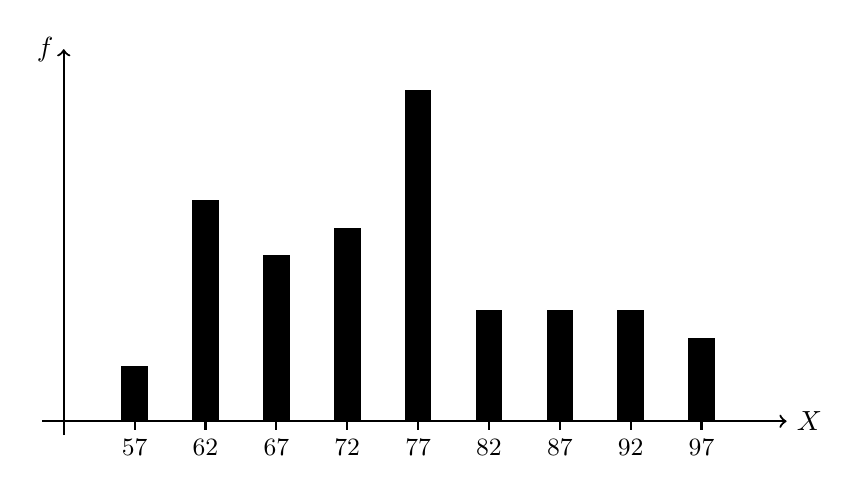
\begin{tikzpicture}[x=0.9cm, y=0.35cm]
  % Axes
  \draw[->, thick] (-0.3, 0) -- (10.2, 0) node[right] {$X$};
  \draw[->, thick] (0, -0.5) -- (0, 13.5) node[left] {$f$};
  
  % Ticks and Bars
  \foreach \i/\h/\lbl in {1/2/57, 2/8/62, 3/6/67, 4/7/72, 5/12/77, 6/4/82, 7/4/87, 8/4/92, 9/3/97} {
    \draw[thick] (\i, 0) -- (\i, -0.3) node[below] {\small\lbl};
    \filldraw[fill=black, draw=black] (\i-0.18, 0) rectangle (\i+0.18, \h);
  }
\end{tikzpicture}

\vspace{0.3em}
\textbf{圖 5-1}
\end{center}

令 $X$ 為將實際成績對應到代表數的隨機變數，則
\begin{align*}
P(X = 57) &= 2/50, & P(X = 62) &= 8/50, & P(X = 67) &= 6/50, \\
P(X = 72) &= 7/50, & P(X = 77) &= 12/50, & P(X = 82) &= 4/50, \\
P(X = 87) &= 4/50, & P(X = 92) &= 4/50, & P(X = 97) &= 3/50.
\end{align*}
現在我們看到抽查一位同學成績在 72 分左右的機率為 7/50，在 77 分左右的機率為 12/50．這樣的分組處理比較符合目的，也是常用的方法． \hfill $\#$

由獨立事件的意義，我們也可以討論隨機變數的獨立性．

\medskip
\noindent\textbf{定義}\quad 設 $(S, P)$ 為機率空間，$X_1, X_2$ 為隨機變數．如果對於任意實數 $x_1, x_2$，$(X_1 = x_1)$ 與 $(X_2 = x_2)$ 皆為獨立事件（在此空事件亦考慮在內，空事件與任意事件，都視為獨立），卽
\[
P[(X_1 = x_1) \cap (X_2 = x_2)] = P(X_1 = x_1) \cdot P(X_2 = x_2)
\]
則稱 $X_1, X_2$ 為（互相）獨立隨機變數．

一般說來，設 $X_1, \dots\dots, X_k$ 為隨機變數．如果對於任意實數 $x_1, \dots\dots, x_k$，下列乘法公式
\begin{align*}
&P[(X_1 = x_1) \cap (X_2 = x_2) \cap \dots\dots \cap (X_k = x_k)] \\
&\quad = P(X_1 = x_1) \cdot P(X_2 = x_2) \cdots\cdots P(X_k = x_k)
\end{align*}
皆成立時，則稱 $X_1, \dots\dots, X_k$ 為（互相）獨立隨機變數．

\medskip
\noindent\textbf{〔例 4〕} 討論例 1 中各隨機變數的獨立性．

\indent\textbf{解}\quad 令 $x_1, x_2, x_3 = 0$ 或 $1$，則
\[
P[(X_1 = x_1) \cap (X_2 = x_2) \cap (X_3 = x_3)] = P(X_1 = x_1) P(X_2 = x_2) P(X_3 = x_3)
\]
恆成立，因此 $X_1, X_2, X_3$ 為獨立隨機變數．

由
\[
P[(X_1 = 1) \cap (X = 2)] = \frac{1}{4} \ne P(X_1 = 1) P(X = 2) = \frac{1}{2} \times \frac{3}{8} = \frac{3}{16}
\]
可知 $X_1$ 與 $X$ 不獨立．同理 $X_2$ 與 $X$，$X_3$ 與 $X$ 亦不獨立．

由 $P[(X = 3) \cap (Y = 0)] \ne P(X = 3) P(Y = 0)$ 知 $X, Y$ 不獨立，用同樣方法可推得 $X$ 與 $Z$；$Y$ 與 $Z$；$X_1$ 與 $Y$；$X_2$ 與 $Y$；$X_2$ 與 $Z$；$X_3$ 與 $Z$ 皆不獨立，而 $X_3$ 與 $Y$；$X_1$ 與 $Z$ 則為獨立． \hfill $\#$

\medskip
\noindent\textbf{〔例 5〕} 調查某社區居民的出生年月，令隨機變數
\begin{align*}
X &\colon \text{姓名} \longrightarrow \text{出生年度，} \\
Y &\colon \text{姓名} \longrightarrow \text{出生月份．}
\end{align*}
則 $X$ 與 $Y$ 應為獨立隨機變數．（在理論上似乎這樣假設才合理，而在實際上可能會有很大出入．我們當然也能作一個人為的例子，使 $X$ 與 $Y$ 不為互相獨立）． \hfill $\#$

\subsubsection*{乙、機率分佈}

隨機變數將樣本空間變換為實數，使得我們能夠將樣本空間上的機率也轉換為實數上的機率，來討論分佈的情形．

\medskip
\noindent\textbf{定義}\quad 設 $(S, P)$ 為機率空間，$X$ 為隨機變數．定義函數
\[
f_X(x) = P(X = x), \quad x \in X(S) \subset \mathbf{R}
\]
$f_X$ 叫做隨機變數 $X$ 的\textbf{機率（密度）函數}．

我們按照機率函數 $f_X$ 的形式分類，一般的機率可以分為下列幾種類型：

\medskip
\noindent\textbf{I. 均等分佈：}設樣本空間 $S = \{a_1, \dots\dots, a_n\}$，機率函數 $P$ 在各樣本點取相同的值，卽 $P(a_j) = \frac{1}{n}, j = 1, \dots\dots, n$．令隨機變數 $X(a_j) = j, j = 1, \dots\dots, n$．則 $X$ 的機率函數為
\[
f_X(j) = \frac{1}{n}.
\]
此函數的圖形為 $n$ 個點如下面左圖所示：

\begin{center}
\begin{minipage}{0.45\textwidth}
\centering
\begin{tikzpicture}[x=0.85cm, y=1.8cm]
  \draw[->, thick] (-0.3, 0) -- (5.2, 0) node[right] {$x$};
  \draw[->, thick] (0, -0.2) -- (0, 1.4) node[left] {$f_X$};
  \draw[thick] (0, 1) -- (-0.15, 1) node[left] {$\dfrac{1}{n}$};
  \draw[thick] (1, 0) -- (1, -0.08) node[below] {$1$};
  \draw[thick] (2, 0) -- (2, -0.08) node[below] {$2$};
  \draw[thick] (3, 0) -- (3, -0.08) node[below] {$3$};
  \draw[dashed, thick] (3.3, 0) -- (4.2, 0);
  \draw[thick] (4.5, 0) -- (4.5, -0.08) node[below] {$n$};
  
  \filldraw[black] (1, 1) circle (2pt);
  \filldraw[black] (2, 1) circle (2pt);
  \filldraw[black] (3, 1) circle (2pt);
  \draw[dashed, thick] (3.2, 1) -- (4.3, 1);
  \filldraw[black] (4.5, 1) circle (2pt);
\end{tikzpicture}
\end{minipage}
\hfill
\begin{minipage}{0.45\textwidth}
\centering
\begin{tikzpicture}[x=0.85cm, y=1.8cm]
  \draw[->, thick] (-0.3, 0) -- (5.2, 0) node[right] {$x$};
  \draw[->, thick] (0, -0.2) -- (0, 1.4) node[left] {$f_X$};
  \draw[thick] (0, 1) -- (-0.15, 1) node[left] {$\dfrac{1}{n}$};
  \draw[thick] (1, 0) -- (1, -0.08) node[below] {$1$};
  \draw[thick] (2, 0) -- (2, -0.08) node[below] {$2$};
  \draw[thick] (3, 0) -- (3, -0.08) node[below] {$3$};
  \draw[dashed, thick] (3.3, 0) -- (4.2, 0);
  \draw[thick] (4.5, 0) -- (4.5, -0.08) node[below] {$n$};
  
  \filldraw[fill=black, draw=black] (1-0.1, 0) rectangle (1+0.1, 1);
  \filldraw[fill=black, draw=black] (2-0.1, 0) rectangle (2+0.1, 1);
  \filldraw[fill=black, draw=black] (3-0.1, 0) rectangle (3+0.1, 1);
  \draw[dashed, thick] (3.2, 1) -- (4.3, 1);
  \filldraw[fill=black, draw=black] (4.5-0.1, 0) rectangle (4.5+0.1, 1);
\end{tikzpicture}
\end{minipage}

\vspace{0.3em}
\textbf{圖 5-2}
\end{center}

為了觀察方便起見，我們常將點改為粗線段，如上面右圖所示，看起來比較清楚．

擲一粒骰子，在班上任意抽選一位同學，以及愛國獎券開獎等都屬於這一類型．

\medskip
\noindent\textbf{II. 伯努利（Bernoulli）分佈：}在此一類型中樣本空間只有兩個樣本點，設
\[
S = \{a, a'\}, \quad P(a) = p, \; 0 < p < 1, \quad P(a') = q = 1 - p.
\]
若令隨機變數 $X(a) = 1, X(a') = 0$．則 $X$ 之機率函數為
\begin{equation}
f_X(1) = p, \quad f_X(0) = q. \label{eq:b5-ch5-1}
\end{equation}
擲一枚公正的硬幣 $\left(p = q = \frac{1}{2}\right)$，自 $m$ 個紅球及 $n$ 個白球（同樣的球）中摸出一球（若以 1 表示摸到紅球，則 $p = \frac{m}{m+n}$，$q = \frac{n}{m+n}$），以及產品的不合格比率，棒球的打擊率，籃球的命中率等等都屬於這一類型．這種只考慮有兩個可能結果，一為成功，一為失敗 的試驗有時就叫做伯努利試驗．

\medskip
\noindent\textbf{III. 二項分佈：（通常叫做伯努利二項分佈）}

若將上項伯努利試驗重複 $n$ 次，並令隨機變數 $X$ 表示基本事件 $a$ 出現的次數，則 $X$ 的機率函數為（設 $p, q$ 如上）
\begin{equation}
f_X(k) = \binom{n}{k} p^k q^{n-k}, \quad k = 0, 1, \dots\dots, n. \label{eq:b5-ch5-2}
\end{equation}
上式右邊恰為下列二項展開式
\[
(p + q)^n = \sum_{k=0}^n \binom{n}{k} p^k q^{n-k}
\]
中的第 $k+1$ 項，所以叫 $X$ 之機率分佈為二項分佈．我們通常用下列符號表示 $b(k; n, p) = \binom{n}{k} p^k q^{n-k} \; (q = 1 - p)$．

\medskip
\noindent\textbf{〔例 6〕} 擲公正的骰子 6 次．令隨機變數 $X$ 表示一點出現的次數，$Y$ 表示二點出現的次數．則機率函數
\[
f_X(k) = f_Y(k) = b\left(k; 6, \frac{1}{6}\right) = \binom{6}{k} \left(\frac{1}{6}\right)^k \left(\frac{5}{6}\right)^{6-k}, \quad k = 0, 1, 2, 3, 4, 5, 6.
\]

\begin{center}
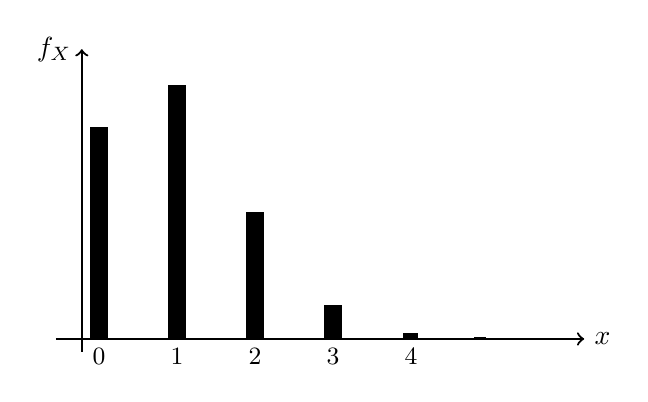
\begin{tikzpicture}[x=1.1cm, y=8cm]
  \draw[->, thick] (-0.3, 0) -- (5.8, 0) node[right] {$x$};
  \draw[->, thick] (0, -0.02) -- (0, 0.46) node[left] {$f_X$};
  
  % Bars for k = 0 to 6
  \filldraw[fill=black, draw=black] (0.2-0.1, 0) rectangle (0.2+0.1, 0.3349);
  \node[below] at (0.2, 0) {\small $0$};
  
  \filldraw[fill=black, draw=black] (1.1-0.1, 0) rectangle (1.1+0.1, 0.4019);
  \node[below] at (1.1, 0) {\small $1$};
  
  \filldraw[fill=black, draw=black] (2.0-0.1, 0) rectangle (2.0+0.1, 0.2009);
  \node[below] at (2.0, 0) {\small $2$};
  
  \filldraw[fill=black, draw=black] (2.9-0.1, 0) rectangle (2.9+0.1, 0.0536);
  \node[below] at (2.9, 0) {\small $3$};
  
  \filldraw[fill=black, draw=black] (3.8-0.08, 0) rectangle (3.8+0.08, 0.0080);
  \node[below] at (3.8, 0) {\small $4$};
  
  \filldraw[fill=black, draw=black] (4.6-0.06, 0) rectangle (4.6+0.06, 0.002);
  
  \filldraw[fill=black, draw=black] (5.3-0.06, 0) rectangle (5.3+0.06, 0.0008);
\end{tikzpicture}

\vspace{0.3em}
\textbf{圖 5-3}
\end{center}

我們還可以算出 $X = j$ 與 $Y = k$ 的積事件，卽恰好出現 $j$ 個一點，$k$ 個二點的機率：
\[
P[(X = j) \cap (Y = k)] = \frac{6!}{j!\, k!\, (6 - j - k)!} \left(\frac{1}{6}\right)^{j+k} \left(\frac{4}{6}\right)^{6-j-k},
\]
\[
j, k = 0, 1, 2, 3, 4, 5, 6; \quad j + k \le 6.
\]
（同學們不難看出上式右邊是多項式展開中一項）．有了上式我們可進一步算出在 $Y = k$ 之下 $X = j$ 的條件機率
\begin{align*}
P[(X = j) \mid (Y = k)] &= P[(X = j) \cap (Y = k)] / P(Y = k) \\
&= P[(X = j) \cap (Y = k)] / f_Y(k) \\
&= \frac{(6 - k)!}{j!\, (6 - j - k)!} \cdot \frac{4^{6-j-k}}{5^{6-k}} = \binom{6 - k}{j} \left(\frac{1}{5}\right)^j \left(\frac{4}{5}\right)^{6-k-j}.
\end{align*}
上式的最後結果又是二項式 $\left(\frac{1}{5} + \frac{4}{5}\right)^{6-k}$ 展開後的第 $j+1$ 項． \hfill $\#$

\medskip
\noindent\textbf{*IV. 布阿松（Poisson）分佈}

在二項分佈的試驗中，若重複的次數 $n$ 非常的大，而機率 $p$ 很小，且 $np = \lambda$ 固定時，則下列近似公式成立：
\begin{equation}
f_X(k) \approx \frac{\lambda^k}{k!} e^{-\lambda}, \quad k = 0, 1, 2, \dots\dots \label{eq:b5-ch5-3}
\end{equation}
式中 $e$ 為常數 $= 2.71828\dots\dots$ 是自然對數的底．上式右邊叫做布阿松分佈，是二項分佈的極限情形（$n \to \infty$ 的情形，導出的過程中要用極限討論，較為複雜，故予省略）．

此類分佈在應用甚為重要，例如在短時間內電話打入的次數或在短時間內到達某一交叉口之車數均近似於此分佈．

\medskip
\noindent\textbf{*〔例 7〕} 設袋中有 1 個紅球，99 個白球（同樣的球），每次採取一球，隨卽放回．若重複採取 100 次，並令 $X$ 表示 100 次中取到紅球的次數．則按二項分佈的機率函數為
\[
f_X(k) = \binom{100}{k} \left(\frac{1}{100}\right)^k \left(\frac{99}{100}\right)^{100-k}, \quad k = 0, 1, \dots\dots, 100.
\]
以及按布阿松分佈的機率函數為（$\lambda = 1$）：
\[
f_X^*(k) = \frac{1}{k!} e^{-1}, \quad k = 0, 1, \dots\dots, 100.
\]
計算結果列表如下：

\begin{center}
\renewcommand{\arraystretch}{1.2}
\begin{tabular}{c|c|c}
\hline\hline
$k$ & $f_X(k)$ & $f_X^*(k)$\phantomsection\label{note:b5-ch5-p150-fxstar}\footnote{【原書註記/校訂】：原書此處表頭印作「$f^{X*}(k)$」，為「$f_X^*(k)$」排版微異之記號，茲予規範化為 $f_X^*(k)$．} \\
\hline
0 & 0.3660 & 0.3679 \\
1 & 0.3697 & 0.3679 \\
2 & 0.1849 & 0.1839 \\
3 & 0.0610 & 0.0613 \\
4 & 0.0149 & 0.0153 \\
5 & 0.0029 & 0.0031 \\
6 & 0.0005 & 0.0005 \\
7 & 0.0001 & 0.0001 \\
8 & 0.0000 & 0.0000 \\
\hline\hline
\end{tabular}
\end{center}
\hfill $\#$

\medskip
\noindent\textbf{*V. 幾何分佈}

設樣本空間 $S = \{a, a'\}$，$P(a) = p, \; 0 < p < 1$，$P(a') = q = 1 - p$．如果無限制重複試驗，令 $X$ 表示首次出現事件 $a$ 的次數，則 $X$ 之機率函數
\begin{equation}
f_X(k) = q^{k-1} p, \quad k = 1, 2, \dots\dots \label{eq:b5-ch5-4}
\end{equation}
對 $k$ 求和，得
\begin{align*}
f_X(1) + f_X(2) + \dots\dots + f_X(k) + \dots\dots &= p + qp + \dots\dots + q^{k-1} p + \dots\dots \\
&= p(1 + q + \dots\dots) = \frac{p}{1 - q} = \frac{p}{p} = 1.
\end{align*}
因為上式形成公比為 $q$ 的幾何級數，故稱 $X$ 為幾何分佈．

\medskip
\noindent\textbf{〔例 8〕} 重複擲一粒公正的骰子，試求在第 6 次始出現一點的機率．

\indent\textbf{解}\quad $f_X(6) = \left(\dfrac{5}{6}\right)^5 \left(\dfrac{1}{6}\right)$\phantomsection\label{note:b5-ch5-p151-px6}\footnote{【原書註記/校訂】：原書此處印作「$P_X(6) = \left(\frac{5}{6}\right)^5 \left(\frac{1}{6}\right)$」，此處係指隨機變數 $X$ 之機率函數值，依全書符號體系宜作 $f_X(6)$，茲予校訂．}． \hfill $\#$

\medskip
\noindent\textbf{**VI. 負二項分佈．}

若重複伯努利試驗，令隨機變數 $X_r$ 表示第 $r$ 個 $a$ 出現的試驗次數．則 $X_r = k \; (k \ge r)$ 卽為恰好在第 $k$ 次試驗時出現第 $r$ 個 $a$ 的事件，因此
\begin{equation}
f_{X_r}(k) = P(X_r = k) = \binom{k-1}{r-1} p^r q^{k-r}, \label{eq:b5-ch5-5}
\end{equation}
\[
r = 1, 2, \dots\dots; \quad k = r, r+1, \dots\dots.
\]
因為到第 $k-1$ 次試驗為止，必須恰已出現 $r-1$ 次 $a$，而在第 $k$ 次必須出現 $a$，所以兩個階段的機率相乘
\[
\binom{k-1}{r-1} p^{r-1} q^{k-r} \times p,
\]
卽得到 (5) 式．

如果我們將二項係數的定義擴展為負整數，卽設 $r, k$ 為自然數，且 $k \ge r$，定義
\[
\binom{-r}{k-r} = \frac{(-r)(-r-1)\cdots\cdots [-r-(k-r)+1]}{(k-r)!}.
\]
而
\begin{align*}
\binom{k-1}{r-1} &= \frac{(k-1)(k-2)\cdots\cdots(k-r+1)}{(r-1)!} \\
&= \frac{(k-1)!}{(r-1)!\, (k-r)!} \\
&= \frac{(k-1)(k-2)\cdots\cdots r}{(k-r)!}
\end{align*}
因此
\[
(-1)^{k-r} \binom{-r}{k-r} = \binom{k-1}{r-1},
\]
(5) 可改寫為
\[
f_{X_r}(k) = \binom{-r}{k-r} p^r (-q)^{k-r},
\]
所以叫做負二項分佈．

\medskip
\noindent\textbf{〔例 9〕} 重複擲一粒公正的骰子，求恰好在第 60 次出現第 10 個么點的機率．

\indent\textbf{解}
\begin{align*}
f_{X_{10}}(60) &= \binom{60-1}{10-1} \left(\frac{1}{6}\right)^{10} \left(\frac{5}{6}\right)^{60-10} \\
&= \binom{59}{9} \left(\frac{1}{6}\right)^{10} \left(\frac{5}{6}\right)^{50}. \tag*{\#}
\end{align*}

% ==============================================================================
% 習題 V-1
% ==============================================================================
\subsubsection*{習題 V-1}\label{sec:b5-ex5-1}

\begin{enumerate}[label=\textbf{\arabic*.}]
  \item 擲公正的骰子三粒，令隨機變數 $X$ 為三粒骰子出現的點數和，試求 $X$ 的機率函數（卽算出 $f_X(3), f_X(4), \dots\dots, f_X(18)$）．

  \item 擲一枚公正的硬幣 10 次，令隨機變數 $X$ 表示出現正面的次數，$Y$ 表示出現反面的次數，試用語言解釋下列各項．
  \begin{enumerate}[(1)]
    \item $(X = 5)$
    \item $(X = 4) = (Y = 6)$
    \item $(X > 5) \cap (Y > 5) = \phi$
    \item $(X \ge 5) \cup (Y \ge 5) = S$（全事件）
  \end{enumerate}

  \item 擲一粒公正的骰子三次，令 $X$ 表示三次出現的點數和，$X_i$ 表示第 $i$ 次出現的點數，$Y$ 表示前兩次出現的點數和，試證：
  \begin{enumerate}[(1)]
    \item $X, X_1$ 不獨立．
    \item $X_1, X_2, X_3$ 互為獨立．
    \item $X, Y$ 不獨立．
    \item $X_1, Y$ 不獨立．
  \end{enumerate}

  \item 將 5 個球任意分配到三個箱子中，令隨機變數 $X$ 表示第一個箱中球數，$Y$ 表示第一、二兩個箱中共有球數，試求：
  \[
  P[(X = a) \cap (Y = b)] \quad \text{及} \quad P(X = a \mid Y = b),
  \]
  \[
  a, b = 0, 1, 2, 3, 4, 5; \; a \le b \quad \text{（請列表）}
  \]

  \item 將 $1, 2, 3$ 三個數字任意排列，共有 6 種情形，假設每種情形的機率為 $1/6$，定義隨機變數 $X$ 及 $Y$ 如下：
  \[
  X(i, j, k) = \begin{cases}
  1 & \text{若 } i < j \\
  0 & \text{其他}
  \end{cases}
  \]
  \[
  Y(i, j, k) = \begin{cases}
  1 & \text{若 } k > i \text{ 及 } k > j \\
  0 & \text{其他}
  \end{cases}
  \]
  \begin{enumerate}[(1)]
    \item 試計算 $P[(X = 1) \cap (Y = 1)]$, $P[(X = 1) \cap (Y = 0)]$, $P[(X = 0) \cap (Y = 1)]$, 及 $P[(X = 0) \cap (Y = 0)]$．
    \item 試證 $X, Y$ 互為獨立．
    \item 你能說明此獨立性的直觀意義嗎？
  \end{enumerate}

  \item \textbf{配對問題．}
  \begin{enumerate}[(1)]
    \item 設有三把外型相同的鎖（卽鑰匙）\phantomsection\label{note:b5-ch5-p153-q6}\footnote{【原書註記/校訂】：原書此題題號下僅有小題編號 (1)，並無 (2)，正文照原書保留小題標號 (1)．}，編為 $1, 2, 3$ 號，若三支鑰匙被混在一起，由三個人各任取一支，去試開一鎖，令隨機變數 $X$ 表示被打開的鎖的個數，試求 $X$ 及其機率函數 $f_X$，樣本點可用 $(x, y, z)$ 表示，其中 $x, y, z = 1, 2, 3$ 且為互異．例如 $(2, 1, 3)$ 表示 2 號鑰匙用 1 號鎖，1 號鑰匙用 2 號鎖，3 號鑰匙開 3 號鎖，只有一個符合，故 $X(2, 1, 3) = 1$．
  \end{enumerate}

  \item 設以全班同學為樣本空間，令隨機變數 $X$ 表示前次月考國文成績，$Y$ 表示英文成績，$Z$ 表示數學成績，試仿照論例 1，求 $f_X, f_Y, f_Z$，並討論 $X, Y, Z$ 的獨立性．

  \item 設某大工廠每天用水量為正常（卽一天用水量在某一定範圍之內）的機率為 $\frac{3}{4}$，令隨機變數 $X$ 表示一週內（以六天計算，自星期一至星期六）用水正常的天數，試求 $f_X(k), k = 0, 1, \dots\dots, 6$．
\end{enumerate}
% ==============================================================================
% § V-2 期望值與方差
% ==============================================================================
\subsection{期望值與方差}\label{sec:b5-5-2}

假設某期愛國獎券發行100萬張，獎額如下：
\begin{center}
\begin{tabular}{rc@{\qquad}cr}
第一特獎 & 1 張 & 獎金 & 50萬元 \\
頭\quad 獎 & 1 張 & 獎金 & 20萬元 \\
二\quad 獎 & 1 張 & 獎金 & 10萬元 \\
三\quad 獎 & 15張 & 獎金 & 2萬元 \\
\multicolumn{2}{c}{\ldots\ldots} & \multicolumn{2}{c}{\ldots\ldots}
\end{tabular}
\end{center}
則每張獎券的平均獎金爲
\[
\frac{1}{10^6} (5 \cdot 10^5 + 2 \cdot 10^5 + 10^5 + 15 \times 2 \cdot 10^4 + \ldots\ldots).
\]
在一般情形，這樣的平均數叫做\textbf{數學期望值}，簡稱爲\textbf{期望值}，現給予定義如下：

\medskip
\noindent\textbf{定義}\quad 設 $(S, P)$ 爲機率空間，$X$ 爲隨機變數，$f_X$ 爲 $X$ 的機率函數．設 $X(S)=\{x_1, \ldots\ldots, x_n\}$，定義
\begin{align}
E(X) &= \sum_{k=1}^n x_k f_X(x_k) \tag{1}\label{eq:b5-5-2-1} \\
&= \sum_{k=1}^n x_k P\{X=x_k\} \tag{$1'$}\label{eq:b5-5-2-1p}
\end{align}
叫做 $X$ 的\textbf{期望值}（$E$ 爲 Expectation 的第一個字母），（有時亦記爲 $\mu$，卽 $\mu=E(X)$，$\mu$ 唸做 $\mathrm{Mu}$）\phantomsection\label{note:b5-ch5-p155-doubled-comma}\footnote{【原書註記/校訂】：原書印作「（有時亦記爲 $\mu$,, 卽 $\mu=E(X)$」，有重疊逗號，茲予更正．}．

若 $S = \{a_1, \ldots\ldots, a_m\}$，則 (1) 也可以寫爲
\begin{equation}\tag{$1''$}\label{eq:b5-5-2-1pp}
E(X) = \sum_{j=1}^m X(a_j) P(a_j)
\end{equation}
由上式可知，若 $X \equiv c$（常數），則得期望值 $\mu = c$．

\medskip
\noindent\textbf{〔例 10〕}求例 1 中各隨機變數的期望值．

\indent\textbf{解}\quad $E(X_1) = 0 \cdot P(X_1=0) + 1 \cdot P(X_1=1) = 0 \cdot \frac{1}{2} + 1 \cdot \frac{1}{2} = \frac{1}{2}$，同理可得
\[
E(X_2) = EX_3 = \frac{1}{2}.
\]
\begin{align*}
E(X) &= 0 \cdot P(X=0) + 1 \cdot P(X=1) + 2 \cdot P(X=2) + 3 \cdot P(X=3) \\
&= 0 \cdot \frac{1}{8} + 1 \cdot \frac{3}{8} + 2 \cdot \frac{3}{8} + 3 \cdot \frac{1}{8} = \frac{3}{2}, \\
E(Y) &= 0 \cdot \frac{1}{4} + 1 \cdot \frac{1}{2} + 2 \cdot \frac{1}{4} = 1, \\
E(Z) &= 0 \cdot \frac{1}{4} + 1 \cdot \frac{1}{2} + 2 \cdot \frac{1}{4} = 1. \tag*{\#}
\end{align*}

\medskip
\noindent\textbf{〔例 11〕}求論例 1 中的平均成績——根據分佈組合成表．

\indent\textbf{解}\quad $\begin{aligned}[t]
EX &= 57 \cdot \frac{2}{50} + 62 \cdot \frac{8}{50} + 67 \cdot \frac{6}{50} + 72 \cdot \frac{7}{50} + 77 \cdot \frac{12}{50} + 82 \cdot \frac{4}{50} + 87 \cdot \frac{4}{50} \\
&\quad + 92 \cdot \frac{4}{50} + 97 \cdot \frac{3}{50} = 75.66.
\end{aligned}$

實際的算術平均值爲 75.36，二者甚爲接近． \hfill \#

\medskip
\noindent\textbf{〔例 12〕}將 $n$ 個球任意分配到三個箱中，令隨機變數 $X$ 表示分配之後空箱子的個數，則
\begin{align*}
f_X(2) &= P(X=2) = \binom{3}{1}\left(\frac{1}{3}\right)^n = \left(\frac{1}{3}\right)^{n-1}, \\
f_X(1) &= P(X=1) = \binom{3}{2}\left(\frac{2}{3}\right)^n - \binom{2}{1}\left(\frac{1}{3}\right)^{n-1} = \frac{2^n - 2}{3^{n-1}}, \\
f_X(0) &= 1 - f_X(1) - f_X(2) = 1 - \frac{2^n - 1}{3^{n-1}}.
\end{align*}
而期望值
\[
EX = 2 \left(\frac{1}{3}\right)^{n-1} + 1 \cdot \frac{2^n - 2}{3^{n-1}} + 0 \cdot \left(1 - \frac{2^n - 1}{3^{n-1}}\right) = \frac{2^n}{3^{n-1}}.
\]
當 $n=1$ 時 $EX=2$，恰有二空箱；$n=2$ 時 $EX=\frac{4}{3}$；$n=3$ 時 $EX=\frac{8}{9}$． \hfill \#

\medskip
由隨機變數及期望值的定義，(1') 或 (1'') 式，我們可以推得下列性質：
\begin{enumerate}[label=\arabic*., leftmargin=2em, itemsep=0.3em]
  \item 設 $X_1, \ldots\ldots, X_r$ 爲隨機變數，則和函數 $X_1 + \ldots\ldots + X_r$ 亦爲一隨機變數（稱爲隨機變數 $X_1, \ldots\ldots, X_r$ 的和）我們有
  \begin{equation}\tag{2}\label{eq:b5-5-2-2}
  E(X_1 + \ldots\ldots + X_r) = E(X_1) + \ldots\ldots + E(X_r).
  \end{equation}
  \item 設 $X$ 爲隨機變數，$a$ 爲任意實數，則
  \begin{align}
  E(X+a) &= EX + a \tag{3}\label{eq:b5-5-2-3} \\
  E(aX) &= aEX \tag{4}\label{eq:b5-5-2-4}
  \end{align}
  〔$(aX)(x) = a(X(x))$，所以 $aX$ 也是一個隨機變數〕
  \item 設 $X_1, X_2$ 爲隨機變數，且 $X_1 \le X_2$，則
  \begin{equation}\tag{5}\label{eq:b5-5-2-5}
  E(X_1) \le E(X_2)
  \end{equation}
  \item 設 $X, Y$ 爲獨立隨機變數，則下列乘法公式
  \begin{equation}\tag{6}\label{eq:b5-5-2-6}
  E(XY) = E(X)E(Y)
  \end{equation}
  〔$XY(x) = X(x)Y(x)$，所以也是一個隨機變數〕\\
  一般地，設 $X_1, X_2, \ldots\ldots, X_r$ 爲獨立隨機變數，則
  \begin{equation}\tag{$6'$}\label{eq:b5-5-2-6p}
  E(X_1 \ldots\ldots X_r) = E(X_1) \ldots\ldots E(X_r)
  \end{equation}
\end{enumerate}

\medskip
\noindent\textbf{證明}\quad 由定義 $(1'')$
\begin{align*}
E(XY) &= \sum_{j=1}^m XY(a_j) P(a_j) \\
&= \sum_{j=1}^m X(a_j) Y(a_j) P(a_j).
\end{align*}
令 $X(S)=\{x_1, \ldots\ldots, x_r\}$，$Y(S)=\{y_1, \ldots\ldots, y_s\}$，則由獨立性得
\[
x_i y_j P[(X=x_i) \cap (Y=y_j)] = x_i y_j P(X=x_i) P(Y=y_j).
\]
由上可知各 $(X=x_i) \cap (Y=y_j)$ 皆非空事件又因 $S = \bigcup_{i, j}[(X=x_i) \cap (Y=y_j)]$ 且各個子集 $[(X=x_i) \cap (Y=y_j)]$ 互不相交，所以每個 $a \in S$ 恰好屬於某一個子集 $(X=x_i) \cap (Y=y_j)$．若 $(X=x_i) \cap (Y=y_j) = \{a_{k_1}, \ldots\ldots, a_{k_t}\}$，則 $X(a_{k_1}) Y(a_{k_1}) P(a_{k_1}) + \ldots\ldots + X(a_{k_t}) Y(a_{k_t}) P(a_{k_t}) = x_i y_j [P(a_{k_1}) + \ldots\ldots + P(a_{k_t})] = x_i y_j P[(X=x_i) \cap (Y=y_j)]$ 因此
\begin{align*}
E(XY) &= \sum_{i=1}^r \sum_{j=1}^s x_i y_j P[(X=x_i) \cap (Y=y_j)] \\
&= \sum_{i=1}^r \sum_{j=1}^s x_i y_j P(X=x_i) P(Y=y_j) \\
&= \sum_{i=1}^r x_i P(X=x_i) \sum_{j=1}^s y_j P(Y=y_j) \\
&= E(X)E(Y).
\end{align*}
對於一般情形，只要利用數學歸納法卽可得證． \hfill \#

\medskip
\noindent\textbf{〔例 13〕}在例 1 中隨機變數 $X_1, X_2, X_3$ 互爲獨立，我們有
\[
EX_1 = EX_2 = EX_3 = 1/2,
\]
故
\[
E(X_1 X_2 X_3) = \left(\frac{1}{2}\right)^3 = \frac{1}{8}.
\]
如果直接計算，則由 $X_1(S) = X_2(S) = X_3(S) = \{0, 1\}$ 以及 $P(X_i=0) = P(X_i=1) = 1/2$ 得
\begin{align*}
E(X_1 X_2 X_3) &= (1 \cdot 1 \cdot 1) P(X_1=1) P(X_2=1) P(X_3=1) \\
&= \left(\frac{1}{2}\right)^3 = \frac{1}{8}. \tag*{\#}
\end{align*}

\medskip
設 $X$ 爲一隨機變數，$EX$ 爲其期望值，若 $X \not\equiv c$，則 $X$ 所取之值與期望值 $EX$ 之間總會產生偏差，我們現在定義 $X$ 的\textbf{方差}（Variance，或稱\textbf{分散}，\textbf{變異量}），用以衡量這種偏差的程度．

\medskip
\noindent\textbf{定義}\quad 設 $(S, P)$ 爲機率空間，$X$ 爲隨機變數，$f_X$ 爲 $X$ 的機率函數，$E(X) = \mu$ 爲其期望值．若 $X(S)=\{x_1, \ldots\ldots, x_n\}$，我們定義 $X$ 的\textbf{方差} $\operatorname{Var} X$ 爲
\begin{equation}\tag{7}\label{eq:b5-5-2-7}
\operatorname{Var} X = E[(X-\mu)^2] = \sum_{k=1}^n (x_k - \mu)^2 f_X(x_k)
\end{equation}
爲方便起見，一般我們用 $\sigma^2$（唸爲 Sigma 平方）來表示 $X$ 的方差\phantomsection\label{note:b5-ch5-p157-fangcha}\footnote{【原書註記/校訂】：原書此頁末句作「來表示 $X$」，未完句且漏標點，次頁（第158頁）首直接承接式 (7) 討論「由期望值 $E$ 的線性性質，我們可將上式化爲」，依文意補足為「來表示 $X$ 的方差」．}．

由期望值 $E$ 的線性性質，我們可將上式化爲
\begin{align}
\operatorname{Var} X &= E[(X-\mu)^2] = E[X^2 - 2\mu X + \mu^2] \nonumber \\
&= E(X^2) - 2\mu E(X) + E(\mu^2) \nonumber \\
&= E(X^2) - 2\mu^2 + \mu^2 = E(X^2) - (EX)^2 \tag{8}\label{eq:b5-5-2-8}
\end{align}
有時利用 (8) 式計算方差比較方便．

由方差的定義可以看出，如果方差的數值微小，則 $X$ 所取的值與期望值 $EX$ 之間有較大偏差的可能性很小，所以一般說來，方差愈大，其分佈情況也愈分散．至於期望值與方差的關係，可以參考 §V-3 中的 (1) 式．

我們現在列出方差的基本性質，前兩項可由定義直接得到：
\begin{enumerate}[label=\arabic*., leftmargin=2em, itemsep=0.3em]
  \item $\operatorname{Var}(X+c) = \operatorname{Var} X$，$c$ 爲任意實數． \hfill $(9)$\label{eq:b5-5-2-9}
  \item $\operatorname{Var}(cX) = c^2 \operatorname{Var} X$，$c$ 爲任意實數． \hfill $(10)$\label{eq:b5-5-2-10}
  \item 設隨機變數 $X, Y$ 互爲獨立，則
  \begin{equation}\tag{11}\label{eq:b5-5-2-11}
  \operatorname{Var}(X+Y) = \operatorname{Var} X + \operatorname{Var} Y
  \end{equation}
  一般地，設 $X_1, \ldots\ldots, X_r$ 互爲獨立，則
  \begin{equation}\tag{12}\label{eq:b5-5-2-12}
  \operatorname{Var}(X_1 + \ldots\ldots + X_r) = \operatorname{Var} X_1 + \ldots\ldots + \operatorname{Var} X_r
  \end{equation}
\end{enumerate}

\medskip
\noindent\textbf{證明}\quad
\begin{align*}
\operatorname{Var}(X+Y) &= E\{[(X+Y)-(EX+EY)]^2\} \\
&= E\{[(X-EX)+(Y-EY)]^2\} \\
&= E\{X^2 + 2XY + Y^2 - 2(X+Y)(EX+EY) \\
&\qquad + (EX^2 + 2EX \cdot EY + EY^2)\} \\
&= E(X^2) + 2E(X)E(Y) + E(Y^2) \\
&\quad - 2E(X+Y)(EX+EY) \\
&\quad + (EX^2 + 2EX \cdot EY + EY^2) \quad \text{（由 $X$ 與 $Y$ 的獨立性）} \\
&= [E(X^2) - (EX)^2] + [E(Y^2) - EY^2] \\
&= \operatorname{Var} X + \operatorname{Var} Y.
\end{align*}
對於一般情形，可用數學歸納法導得．

\medskip
\noindent\textbf{注意}\quad 方差的加法公式要用到隨機變數的獨立性，而期望值的加法公式中則不需要．

\medskip
\noindent\textbf{〔例 14〕}擲公正的骰子一粒，令隨機變數 $X$ 表示出現點數．求 $EX$ 及 $\operatorname{Var} X$．

\indent\textbf{解}\quad $X(S)=\{1, 2, 3, 4, 5, 6\}$，$f_X(k)=1/6$．
\begin{align*}
EX &= \sum_{k=1}^6 \frac{k}{6} = 7/2, \quad E(X^2) = \sum_{k=1}^6 \frac{k^2}{6} = \frac{91}{6}, \\
\operatorname{Var} X &= E(X^2) - (EX)^2 = \frac{91}{6} - \left(\frac{7}{2}\right)^2 = \frac{35}{12}.
\end{align*}
這個問題中的隨機變數爲均等分佈，故偏差不小，（如果機率分佈集中在期望值附近，則偏差較小）． \hfill \#

\medskip
下面列出前節中所提到的各種類型，隨機變數的期望值及方差，供大家參考．

\begin{center}
\renewcommand{\arraystretch}{1.5}
\begin{tabular}{|c|l|c|c|}
\hline
$X$ & \multicolumn{1}{c|}{$f_X(k)$} & $EX$ & $\operatorname{Var} X$ \\
\hline
I. 均等分佈 & $\dfrac{1}{n}, \quad k = 1, \ldots\ldots, n$ & $\dfrac{n+1}{2}$ & $\dfrac{n^2-1}{12}$ \\
\hline
II. 伯努利分佈 & $\begin{aligned}&f_X(1)=p, f_X(0)=q \\ &0 < p < 1, q = 1-p\end{aligned}$ & $p$ & $p(1-p)$ \\
\hline
III. 二項分佈 & $\dbinom{n}{k} p^k q^{n-k}, \quad k = 0, 1, \ldots\ldots, n$ & $np$ & $np(1-p)$ \\
\hline
$*$IV. 布阿松分佈 & $\dfrac{\lambda^k}{k!} e^{-\lambda}, \quad k = 0, 1, \ldots\ldots$ & $\lambda$ & $\lambda$ \\
\hline
$*$V. 幾何分佈 & $q^{k-1}p, \quad k = 1, 2, \ldots\ldots$ & $\dfrac{1}{p}$ & $\dfrac{1-p}{p^2}$ \\
\hline
$**$VI. 負二項分佈 & $\begin{aligned}&\binom{k-1}{r-1} p^r q^{k-r} \\ &r=1, 2, \ldots\ldots; \; k=r, r+1, \ldots\ldots\end{aligned}$ & $\dfrac{r}{p}$ & $\dfrac{r(1-p)}{p^2}$ \\
\hline
\end{tabular}
\end{center}

上表中的結果有些可以直接算出，有些卻要利用一些等式才能算出．

\medskip
\noindent\textbf{〔例 15〕}擲一枚公正的硬幣10次，令隨機變數 $X$ 表示出現正面的次數．求 $EX$ 及 $\operatorname{Var} X$．

\indent\textbf{解}\quad $X$ 的機率函數爲
\[
f_X(k) = \binom{10}{k} \left(\frac{1}{2}\right)^{10}, \quad k = 0, 1, \ldots\ldots, 10.
\]
由上表中公式得
\[
EX = \frac{10}{2} = 5, \quad \operatorname{Var} X = 10 \cdot \frac{1}{2}\left(1 - \frac{1}{2}\right) = \frac{10}{4}. \tag*{\#}
\]

% ==============================================================================
% 習題 V-2
% ==============================================================================
\subsubsection*{習題 V-2}

\begin{enumerate}[label=\arabic*., leftmargin=2em, itemsep=0.5em]
  \item 將 5 個球任意分配\phantomsection\label{note:b5-ch5-p160-fenpei}\footnote{【原書註記/校訂】：原書印作「分取到三個箱子中」，依文義及後句「分配後空箱子的個數」，顯為「分配」之訛，茲予校訂．}到三個箱子中，令隨機變數 $X$ 表示分配後空箱子的個數，試求機率函數 $f_X$ 及 $X$ 的期望值．
  \item 擲一枚公正硬幣10次，定義隨機變數 $X_i \, (i = 1, 2, \ldots\ldots, 10)$ 如下：
  \[
  X_i = \begin{cases}
  1 & \text{若第 $i$ 次出現正面} \\
  0 & \text{其他}
  \end{cases}
  \]
  試求 $E(X_1+X_2+\ldots\ldots+X_{10})$ 及 $E(X_1 X_2 \ldots\ldots X_{10})$．
  \item 擲兩粒公正的骰子，令 $X$ 表示出現的點數和，試求期望值 $EX$ 及方差 $\operatorname{Var} X$．
  \item \begin{enumerate}[label=(\arabic*), itemsep=0.3em, topsep=0.2em]
    \item 自 $\{1, 2, 3, 4, 5, 6, 7, 8, 9, 10\}$ 中任取一數（卽設各數被取機會相等）．試求期望值及方差（可取隨機變數 $X(k)=k, k=1, 2, \ldots\ldots, 10$）．
    \item 同上小題，但改自 $\{1, 2, 3, \ldots\ldots, 100\}$ 中取出．
  \end{enumerate}
\end{enumerate}
% ==============================================================================
% *§ V-3 大數法則
% ==============================================================================
\subsection[大數法則]{大數法則\protect\footnote{* 社會組可略去不授，留供參考．}}\label{sec:b5-5-3}

在本節中我們將討論大量重複試驗的結果與機率的關係，導出幾個基本的有用的定理\phantomsection\label{note:b5-ch5-p160-typo}\footnote{【原書註記/校訂】：原書作「幾個基本的有用的定理」，疑為「幾個基本而有用的定理」之筆誤，此處照原文錄入．}．

我們首先證明柴比雪夫 (Tchebychev) 不等式：

\medskip
\noindent\textbf{〔柴比雪夫不等式〕}\quad 設 $(S, P)$ 為有限機率空間，$X$ 為任一隨機變數，則對於任意 $\varepsilon > 0$，下列不等式成立
\begin{equation}
P\{|X - EX| \ge \varepsilon\} \le \frac{\Var X}{\varepsilon^2} \tag{1}\label{eq:b5-5-3-1}
\end{equation}

\noindent\textbf{**證明}\quad 設 $f_X$ 為 $X$ 的機率函數，並令
\[
A = \{x \mid x \in X(S) \text{ 且 } |x - EX| \ge \varepsilon\}.
\]
則
\[
P\{|X - EX| \ge \varepsilon\} = \sum_{x \in A} f_X(x).
\]
在 $A$ 中的任一個 $x$，
\[
\frac{|x - EX|}{\varepsilon} \ge 1
\]
恆成立．所以
\begin{align*}
\sum_{x \in A} f_X(x) &\le \frac{1}{\varepsilon^2} \sum_{x \in A} (x - EX)^2 f_X(x) \\
&\le \frac{1}{\varepsilon^2} \sum_{x \in X(S)} (x - EX)^2 f_X(x) \\
&= \frac{\Var X}{\varepsilon^2}. \tag*{\#}
\end{align*}

這個不等式的意義表示隨機變數 $X$ 取值與期望值的偏差超過 $\varepsilon$ 的機率不超過 $\frac{\Var X}{\varepsilon^2}$．式中 $\Var X$ 為定數，因此 $\varepsilon$ 愈大，卽偏差愈大時的機會則愈小．

\medskip
\noindent\textbf{〔例 16〕}\quad 擲一枚公正的硬幣 10 次，令隨機變數 $X$ 表示出現正面的次數．則
\[
EX = 5, \quad \Var X = \frac{5}{2} \quad \text{（見例 15）}.
\]
因此柴比雪夫不等式為，
\[
P\{|X - 5| \ge \varepsilon\} \le \frac{5}{2\varepsilon^2}.
\]
$\varepsilon = 1$ 時 $P\{|X - 5| \ge 1\} \le \frac{5}{2}$，右端大於 1，所以我們不能由此不等式得到什麼結論．

$\varepsilon = 2$ 時，$\frac{5}{2 \cdot 2^2} = \frac{5}{8} < 1$，$P\{|X - 5| \ge 2\} \le \frac{5}{8}$，由此可知 $X$ 取值 $0, 1, 2, 3, 7, 8, 9, 10$ 的機率不超過 $5/8$．

$\varepsilon = 3$ 時，$\frac{5}{2 \cdot 3^2} = \frac{5}{18} < 1$，$P\{|X - 5| \ge 3\} \le \frac{5}{18}$，故 $X$ 取值 $0, 1, 2, 8, 9, 10$ 的機率不超過 $\frac{5}{18}$．

$\varepsilon = 5$ 時，$\frac{5}{2 \cdot 5^2} = \frac{1}{10} < 1$，$X$ 取值 $0, 10$ 的機率不超過 $\frac{1}{10}$．實際上 $f_X(0) + f_X(10) = \left(\frac{1}{2}\right)^9 < \frac{1}{10}$． \hfill\#

\medskip
\noindent\textbf{〔柴比雪夫定理〕}\quad 設 $X_1, X_2, \dots$ 為一敍列互相獨立的隨機變數，且其方差有共同界限，卽 ($C$ 為常數)
\[
\Var X_k \le C, \quad k = 1, 2, \dots,
\]
則對於任意 $\varepsilon > 0$，下列極限成立
\begin{equation}
\lim_{n \to \infty} P\left\{ \left| \frac{1}{n}\sum_{k=1}^n X_k - \frac{1}{n}\sum_{k=1}^n EX_k \right| < \varepsilon \right\} = 1 \tag{2}\label{eq:b5-5-3-2}
\end{equation}

\noindent\textbf{**證明}\quad 由假設 $X_1, \dots, X_n$ 為互相獨立，則由方差的基本性質（上節中 (11) 及 (12) 式）得
\begin{align*}
\Var\left(\frac{1}{n}\sum_{k=1}^n X_k\right) &= \frac{1}{n^2}\sum_{k=1}^n \Var X_k \\
&\le \frac{1}{n^2}\sum_{k=1}^n C = \frac{1}{n^2} nC.
\end{align*}
因此
\[
\Var\left(\frac{1}{n}\sum_{k=1}^n X_k\right) \le \frac{C}{n}.
\]
應用柴比雪夫不等式，得
\begin{align*}
P\left\{ \left| \frac{1}{n}\sum_{k=1}^n X_k - \frac{1}{n}\sum_{k=1}^n EX_k \right| < \varepsilon \right\} &\ge 1 - \frac{\Var\left(\frac{1}{n}\displaystyle\sum_{k=1}^n X_k\right)}{\varepsilon^2} \\
&\ge 1 - \frac{C}{n\varepsilon^2}.
\end{align*}
令 $n \to \infty$，則
\[
\lim_{n \to \infty} P\left\{ \left| \frac{1}{n}\sum_{k=1}^n X_k - \frac{1}{n}\sum_{k=1}^n EX_k \right| < \varepsilon \right\} \ge 1,
\]
但機率數值不超過 1，故上式應取等號，定理得證． \hfill\#

這個定理表示一敍列獨立隨機變數的平均偏差小於 $\varepsilon$（$\varepsilon$ 為任意正數）的機率會趨於 1．

下面的定理是柴比雪夫定理的特別情形．

\medskip
\noindent\textbf{〔伯努利 Bernoulli 定理〕}\quad 作一敍列獨立的重複試驗，令隨機變數 $X$ 表示事件 $A$ 在 $n$ 次試驗中出現的次數，$p$ 為在每一次試驗中 $A$ 出現的機率，卽 $p = P(A)$．則對於任意 $\varepsilon > 0$，
\begin{equation}
\lim_{n \to \infty} P\left\{ \left| \frac{X}{n} - p \right| < \varepsilon \right\} = 1 \tag{3}\label{eq:b5-5-3-3}
\end{equation}

\noindent\textbf{**證明}\quad 定義隨機變數 $X_k$ 如下：
\[
X_k = \begin{cases} 1, & \text{在第 $k$ 次試驗中 $A$ 出現；} \\ 0, & \text{在第 $k$ 次試驗中 $A$ 未出現．} \end{cases}
\]
我們有
\[
X = X_1 + \cdots\cdots + X_n \quad (n \text{ 次試驗中 $A$ 出現的次數})
\]
因為
\[
EX_k = p, \quad \Var X_k = pq \le \frac{1}{4}
\]
應用柴比雪夫定理卽得 (3) 式． \hfill\#

這個定理的統計意義如下：

\begin{center}
\begin{tikzpicture}[scale=1.0, >=stealth]
  % Axes
  \draw[->, thick] (-0.3, 0) -- (7.0, 0) node[right] {$n$};
  \draw[->, thick] (0, -0.3) -- (0, 4.2) node[above] {$\dfrac{1}{n}\displaystyle\sum_{i=1}^n X_i$};
  
  \node[below left] at (0, 0) {$0$};
  
  % Parameters
  \def\p{2.1}
  \def\eps{0.8}
  
  % Horizontal bands
  \draw[thick] (0, \p + \eps) -- (6.2, \p + \eps);
  \draw[thick] (0, \p) -- (6.2, \p);
  \draw[thick] (0, \p - \eps) -- (6.2, \p - \eps);
  
  % Tick labels on y-axis
  \node[left] at (0, \p + \eps) {$p + \varepsilon$};
  \node[left] at (0, \p) {$p$};
  \node[left] at (0, \p - \eps) {$p - \varepsilon$};
  
  % Vertical line at n = N
  \def\xN{5.2}
  \draw[thick] (\xN, 0) -- (\xN, 3.8) node[above] {$n = N$};
  \node[below] at (\xN, 0) {$N$};
  
  % Sample realization points on line n = N
  % Inside the strip:
  \filldraw (\xN, \p + 0.5) circle (1.8pt);
  \filldraw (\xN, \p + 0.2) circle (1.8pt);
  \filldraw (\xN, \p - 0.2) circle (1.8pt);
  \filldraw (\xN, \p - 0.5) circle (1.8pt);
  % Outside the strip:
  \filldraw (\xN, \p + \eps + 0.45) circle (1.8pt);
  \filldraw (\xN, \p - \eps - 0.45) circle (1.8pt);
\end{tikzpicture}
\end{center}

隨機變數 $X = \sum_{i=1}^n X_i$ 表示 $n$ 次中出現 $A$ 之次數，而隨機變數 $\frac{1}{n}\sum_{i=1}^n X_i$ 表示 $n$ 次中出現 $A$ 之比率．(3)式之意義可解釋如下：固定 $\varepsilon > 0$（甚小），取 $n = N$，\phantomsection\label{note:b5-ch5-p164-comma}\footnote{【原書註記/校訂】：原書印作「取 $n = N$，，」，多一逗號，此處校正為單個逗號．}若 $N$ 充分大時，由(3)可知
\begin{equation}
P\left(p - \varepsilon < \frac{1}{N}\sum_{i=1}^N X_i < p + \varepsilon\right) \tag{$3'$}\label{eq:b5-5-3-3prime}
\end{equation}
接近於 1．我們先獨立試驗 $N$ 次可得一組結果，設為 $x_1^{(1)}, \allowbreak x_2^{(1)}, \allowbreak \dots, \allowbreak x_N^{(1)}$（卽 $X_1, \allowbreak X_2, \allowbreak \dots, \allowbreak X_N$ 之實現值），而出現 $A$ 之比率為
\[
\bar{x}^{(1)} = \frac{1}{N}\sum_{i=1}^N x_i^{(1)} \quad \left(\text{卽 } \frac{1}{N}\sum_{i=1}^N x_i \text{ 之實現值}\right),
\]
再重新獨立試驗 $N$ 次得另一組結果，設為 $x_1^{(2)}, x_2^{(2)}, \dots, x_N^{(2)}$．而出現 $A$ 之比率為
\[
\bar{x}^{(2)} = \frac{1}{N}\sum_{i=1}^N x_i^{(2)}.
\]
如此重複 $m$ 次，可得 $m$ 個比值：
\[
\bar{x}^{(1)} = \frac{1}{N}\sum_{i=1}^N x_i^{(1)}, \dots\dots, \bar{x}^{(m)} = \frac{1}{N}\sum_{i=1}^N x_i^{(m)},
\]
我們將這些點描在上圖中 $n = N$ 直線上時，由 $(3')$ 可知這些點落在帶 $L_1 L_2$\phantomsection\label{note:b5-ch5-p164-strip}\footnote{【原書註記/校訂】：原書正文提及「落在帶 $L_1 L_2$ 之外」，圖中未標注符號 $L_1, L_2$，依文意係指由直線 $y = p + \varepsilon$ 與 $y = p - \varepsilon$ 所界定之水平帶狀區域．} 之外者不多．例如若
\[
P\left(p - \varepsilon < \frac{1}{N}\sum_{i=1}^N X_i < p + \varepsilon\right) = \frac{95}{100}
\]
時\phantomsection\label{note:b5-ch5-p164-rv}\footnote{【原書註記/校訂】：原書此處機率算式中將隨機變數誤印為小寫字母 $x_i$（即 $P(p-\varepsilon < \frac{1}{N}\sum_{i=1}^N x_i < p+\varepsilon)$），此處依前後文及 $(3')$ 式校訂為大寫 $X_i$．}，則大致可說平均 100 個 $\bar{x}^i$ 中只有 5 個落在帶 $L_1 L_2$ 之外\phantomsection\label{note:b5-ch5-p164-xi}\footnote{【原書註記/校訂】：原書印為「$\bar{x}^i$」，即上文之各組實現比值 $\bar{x}^{(1)}, \dots, \bar{x}^{(m)}$．}．如果 $p$ 為未知時，因 $\varepsilon > 0$ 可以取得任意小，故 $N$ 充分大時（卽實驗次數充分大時），以實驗結果求出之 $\bar{x} = \frac{1}{N}\sum_{i=1}^N x_i$ 來推測 $p$ 值是很可靠的（因為推測錯誤的機會不大），這也就是以下所說的大數法則．

\medskip
\noindent\textbf{【論例 2】}\quad 投一枚不公正的銅錢，出現正面之機率如何推測之問題，可根據上述伯努利定理，將此銅錢試投 $N$ 次，如果正面出現 $M$ 次，就以 $\frac{M}{N}$ 推測正面出現的機率 $p$．此種推測方法當 $N$ 充分大時是非常可靠的．

\medskip
\noindent\textbf{〔例 17〕}\quad 十八世紀法國自然科學家 Buffon 丟銅板 4040 次，得正面 2048 次，比值為 0.507．英國統計學家 Karl Pearson 丟銅板 12000 次得 6019 次正面，比值為 0.5016．他在另一次試驗\phantomsection\label{note:b5-ch5-p165-extra}\footnote{【原書註記/校訂】：原書印作「他在另一次值試驗」，多一「值」字，此處校去贅字．}丟銅板 24000 次，得 12012 次正面，此次的比值為 0.5005．這些銅板可判定為公正的銅板，卽出現正面的機率 $p = 0.5$\phantomsection\label{note:b5-ch5-p165-p}\footnote{【原書註記/校訂】：原書印作大寫「$P = 0.5$」，依文意為理論機率 $p = 0.5$；句末漏標點，此處補上句號．}．他們試驗的結果與伯努利定理的主張相當符合．

\begin{center}
\begin{tabular}{ccccc}
\hline
\textbf{試驗者} & \textbf{試驗次數 $n$} & \textbf{正面次數 $X$} & \textbf{相對頻率（比值）$X/n$} & \textbf{理論機率 $p$} \\
\hline
Buffon & $4040$ & $2048$ & $0.507$ & $0.5$ \\
Karl Pearson & $12000$ & $6019$ & $0.5016$ & $0.5$ \\
Karl Pearson & $24000$ & $12012$ & $0.5005$ & $0.5$ \\
\hline
\end{tabular}
\end{center}

由伯努利定理我們可以推得下列大數法則：

\medskip
\noindent\textbf{〔大數法則〕}\quad 設事件 $A$ 的機率為 $p$，並令 $X$ 表示 $n$ 次重複試驗中 $A$ 出現次數，則對於任意 $\varepsilon > 0$ 及 $\delta > 0$，必可取得自然數 $N$，使得當 $n \ge N$ 時
\begin{equation}
P\left\{\left|\frac{X}{n} - p\right| \ge \varepsilon\right\} < \delta \tag{4}\label{eq:b5-5-3-4}
\end{equation}

大數法則實際上就是伯努利定理的另一種敍述，說明如下：(3)式表示大量重複試驗時 $\frac{X}{n}$ 與 $p$ 的偏差小於 $\varepsilon$ 的機率會接近到 1，反過來說，$\frac{X}{n}$ 與 $p$ 的偏差超過 $\varepsilon$ 的機率就會接近到 0，而這就是(4)式的意義．

下面的定理是伯努利定理對於同一事件，但在每次試驗中機率不同的特別情形．

\medskip
\noindent\textbf{〔布阿松 Poisson 定理〕}\quad 作一敍列獨立試驗．設事件 $A$ 在第 $k$ 次試驗中出現的機率為 $p_k$，令隨機變數 $X$ 表示 $n$ 次試驗中 $A$ 出現的次數．則
\begin{equation}
\lim_{n \to \infty} P\left\{\left|\frac{X}{n} - \frac{p_1 + \cdots\cdots + p_n}{n}\right| < \varepsilon\right\} = 1 \tag{5}\label{eq:b5-5-3-5}
\end{equation}

\noindent\textbf{**證明}\quad 定義隨機變數 $X_k$ 如下：
\[
X_k = \begin{cases} 1, & \text{在第 $k$ 次試驗中 $A$ 出現，} \\ 0, & \text{在第 $k$ 次試驗中 $A$ 未出現．} \end{cases}
\]
則 $X = X_1 + \cdots\cdots + X_n$，且有
\[
EX_k = p_k, \quad \Var X_k = p_k q_k \le \frac{1}{4} \quad (q_k = 1 - p_k)
\]
代入(2)式卽得到(5)式． \hfill\#

我們現在回到柴比雪夫不等式 (1)\phantomsection\label{note:b5-ch5-p166-ineq1}\footnote{【原書註記/校訂】：原書印作「柴比雪夫不等(1)式」，漏「式」字，校訂為「柴比雪夫不等式 (1)」．}．如果在其中令 $X$ 表示 $n$ 次重複試驗中事件 $A$ 出現的次數，並設 $A$ 在每次試驗中出現的機率為 $p$ ($0 < p < 1$)．由 \S\,V-2 的表中查出 $EX = np$, $\Var X = npq$，代入 (1) 式得
\[
P\{|X - np| \ge \varepsilon\} \le \frac{npq}{\varepsilon^2}.
\]
上式可以改寫為
\begin{equation}
P\left\{\left|\frac{X}{n} - p\right| \ge \varepsilon\right\} \le \frac{pq}{n\varepsilon^2} \tag{6}\label{eq:b5-5-3-6}
\end{equation}
這是有關大數法則的另一種簡單形式\phantomsection\label{note:b5-ch5-p166-wlln}\footnote{【原書註記/校訂】：由 (6) 式可知，當 $n \to \infty$ 時，$\frac{pq}{n\varepsilon^2} \longrightarrow 0$，故 $P\left\{\left|\frac{X}{n} - p\right| \ge \varepsilon\right\} \longrightarrow 0$（即相對頻率依機率收斂於理論機率 $p$），此即弱大數法則之定量上界形式．}，對於(4)式中的 $\delta$ 我們取
\[
N \ge \frac{pq}{\varepsilon^2 \delta}
\]
即可．

\medskip
\noindent\textbf{〔例 18〕}
\begin{enumerate}[(i), leftmargin=2.5em, itemsep=0.5em]
  \item 重複丟一枚公正的銅板，令 $X$ 表示 $n$ 次中出現正面次數，問應丟多少次可使 $\frac{X}{n}$ 與 $p = \frac{1}{2}$ 的偏差超過 $0.01$ 的機率小於 $0.01$？\phantomsection\label{note:b5-ch5-p166-p}\footnote{【原書註記/校訂】：原書題幹印作大寫「$P = \frac{1}{2}$」，此處校訂為小寫「$p = \frac{1}{2}$」以與前後文記號統一．}

  \noindent\textbf{解}\quad 利用(6)式，令 $\varepsilon = 0.01, \delta = 0.01$，則可取
  \[
  N \ge \frac{pq}{\varepsilon^2 \delta} = \frac{1}{4} \cdot \frac{1}{(0.01)^2 (0.01)} = \frac{1}{4} \cdot 10^6 = 25 \cdot 10^4.
  \]
  大家會注意到，只要 $N \ge 25 \times 10^4$，則一定可保證 $\frac{X}{n}$ 與 $\frac{1}{2}$ 之差超過 $0.01$ 的機率小於 $0.01$，這並不意味著 $N$ 非 $25 \times 10^4$ 不可．或許 $N$ 不須那麼大，便可達到這一目的．

  \item 重複擲一粒骰子，令 $X$ 表示 $n$ 次中出現一點的次數，問應擲多少次可使 $\frac{X}{n}$ 與 $p = \frac{1}{6}$ 的偏差超過 $0.01$ 的機率小於 $0.01$？

  \noindent\textbf{解}\quad 令 $\varepsilon = 0.01, \delta = 0.01$，則可取
  \[
  N \ge \frac{pq}{\varepsilon^2 \delta} = \frac{1}{6} \cdot \frac{5}{6} \cdot 10^6 = \frac{5}{36} \cdot 10^6.
  \]
\end{enumerate}

在這個例子中所應取的 $N$ 都非常大，這只是根據理論的推斷要求，實際上只要重複相當多次，$\frac{X}{n}$ 與 $p$ 卽已非常接近\phantomsection\label{note:b5-ch5-p167-p}\footnote{【原書註記/校訂】：原書此處印作大寫「$P$」，依文意校為機率參數「$p$」．}，大家可以由前面所說的 Buffon 與 Pearson 的試驗結果看到，偏差都在 $\varepsilon = 0.01$ 之內．
